%%%%%%%%%%%%%%%%%%%%%%
\section{Evaluation}
%%%%%%%%%%%%%%%%%%%%%%

In this section, we profile various aspects of our PIFO design to justify our design choices and demonstrate its capability to achieve line rate performance. We use a  200MHz reference clock in these evaluations.

\subsection{Priority Queue Evaluation}

As explained in Section~\ref{sec:priority-queue}, the priority queue consists of a single skip list and a cache. It is designed to satisfy two properties:
\begin{enumerate}
  \item Packet descriptors can be enqueued at less than line rate
  \item Packet descriptors can be dequeued from the head at line rate
\end{enumerate}

The following sections describe experiments that allow us to characterize the enqueue and dequeue performance of a single priority queue.

\subsubsection*{Effect of Fill Level}
Descriptors can be enqueued into the cache every other clock cycle. The main factor that drives the rate at which descriptors can be enqueued into the skip list is the number of memory operations that are required to find the appropriate insertion location, which increases logarithmically with the number of the descriptors in the skip list. We define the fill level as the number of descriptors in both the skip list and the cache.

Figure \ref{fig:fill_level} shows the effect of the fill level on both the enqueue and the dequeue latency, that is, the number of clock cycles required to complete each of these operations. This experiment uses a skip list with a capacity of 2048 elements (using 12 levels) and 16- entry cache. Each average and maximum is computed over 100 samples. As expected, the enqueue latency increases logarithmically with the number of descriptors and the maximum possible enqueue latency is 130 clock cycles, which agrees with the theoretical maximum given by equation \ref{worst-case-insert_eqn}, with $L = 12$, $T_{Rd}$ = 2, $T_{Wr}$ = 1, $K_{1}$ = 3, and $K_{2}$ = 7.

This result constrains two additional aspects of the design:
\begin{enumerate}
  \item The minimum size of the output register to ensure that it has enough capacity to avoid running empty during the longest possible enqueue operation into the skip list.
    \item The number of priority queues that must be used in parallel in order to support enqueue operations at line rate.
\end{enumerate}

All packets used in this experiment are 64B in length, which take 2 cycles to transfer using our 32B data-path. The dequeue latency plot shows that these 64B packets can be removed in three to five cycles depending on whether the dequeue operation is directly preceded by an insertion into the register cache. This is more than fast enough to meet our 13.44 cycle deadline for 10Gb/s operation.

\begin{figure}[!h]
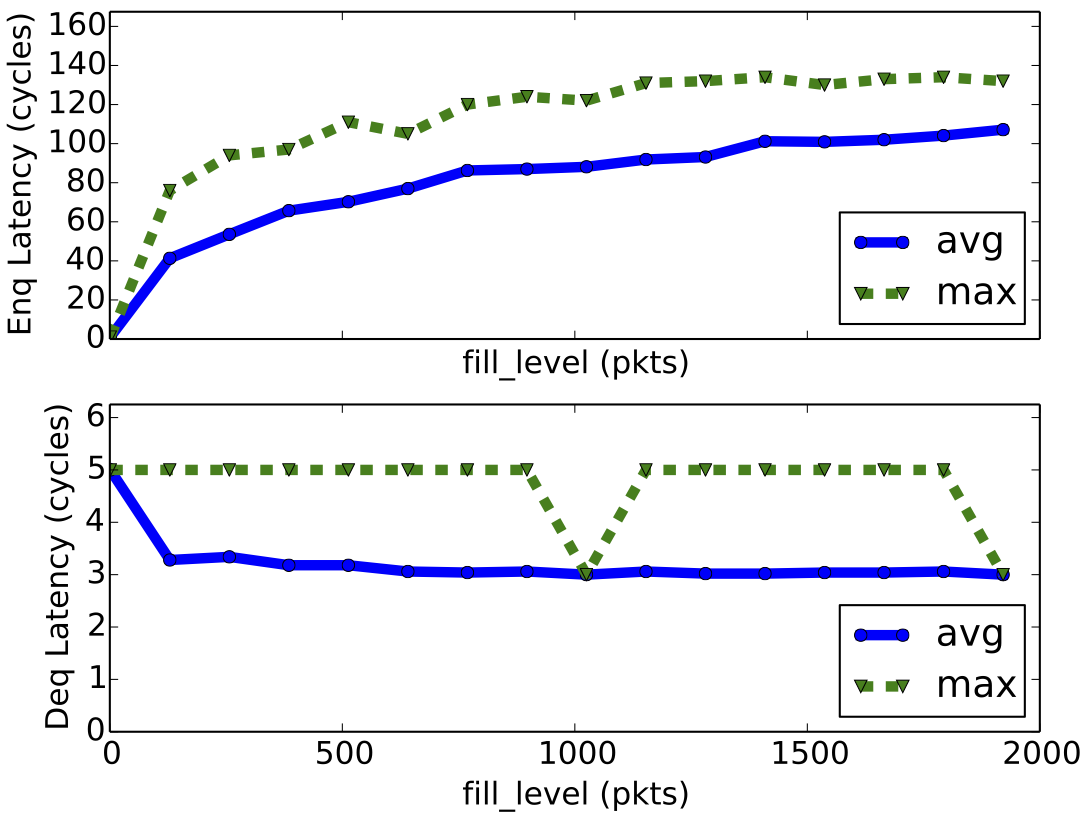
\includegraphics[width=1\linewidth]{figures/eval/enq_deq_v_fill_level}
\caption{Effect on the enqueue and dequeue latencies when the number of entries in the priority queue increases.}
\label{fig:fill_level}
\end{figure}

\subsubsection*{Sizing the Output Register}
The output register must be large enough to satisfy two constraints:
\begin{enumerate}
  \item Large enough to absorb the variations in the rate at which it is being filled by the background process that is replenishing it with descriptors from the skip list.
  \item Large enough to be able to hold enough descriptors such that it will not run empty when the longest possible skip list insertion begins and replenishment from the skip list temporarily stops.
\end{enumerate}

Both of these conditions must be met in order to guarantee that the scheduler will remain work conserving under all conditions. 

To satisfy the first constraint, we must be able to bound the rate at which descriptors are dequeued from the skip list and inserted into the output register. Fortunately, the deterministic structure of the skip list allows us to do exactly that. The maximum number of clock cycles required to dequeue an element from the head of the skip list is directly related to the number of levels in which the head element is present ($L$). This relationship is given by the following expression,

\begin{equation}\label{worst-case-remove_eqn}
T_{Rd} \times L + K_{3}
\end{equation}
where:\\
\indent $T_{Rd}$ = node read time\footnote{Writes are performed as well but they do not contribute to the latency because they are performed in parallel with the reads} = 2 clock cycles\\
\indent $K_{3}$ = processing overhead = 6 clock cycles\\

The deterministic skip list structure property enforces that the node heights, i.e. the number of levels in which they appear, are well distributed. This means that the dequeue rate from the skip list is mostly constant. Figure \ref{fig:out_reg_size} shows the fill level of the output register during an experiment where the skip list starts out filled with 2K descriptors and is then drained at a rate of one descriptor every 12 cycles, faster than line rate. We see that the number of descriptors in the output register never drops by more than two indicating that it is indeed being filled faster than it is being drained. Our measurements indicate that on average, the head element can be removed from the skip list in 8 cycles and in the worst case it can take up to 30 cycles, just over two minimum packet times.

\begin{figure}[!ht]
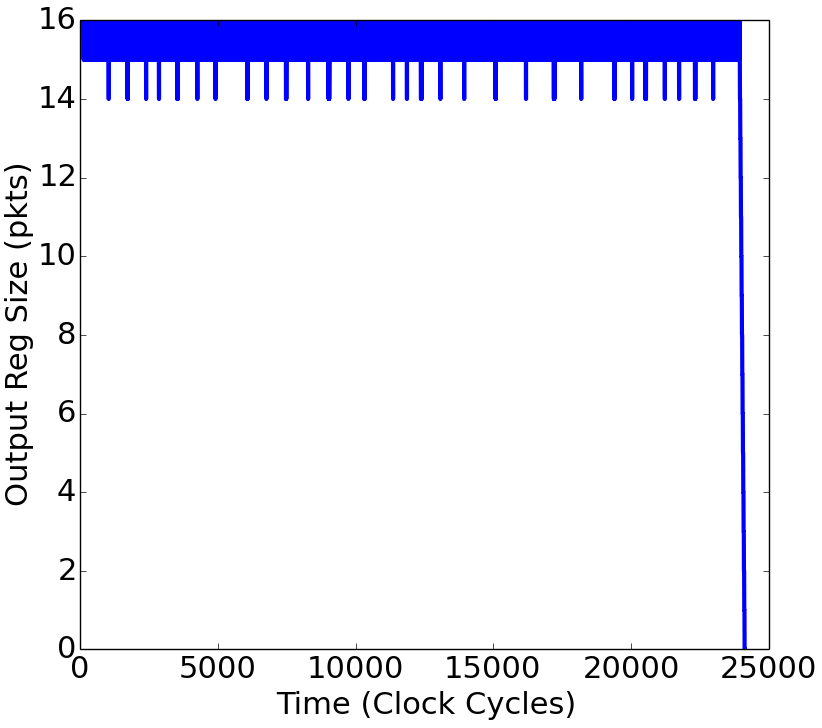
\includegraphics[width=1\linewidth]{figures/eval/out_reg_size}
\caption{The fill level of the output register while draining a skip list with 2K descriptors.}
\label{fig:out_reg_size}
\end{figure}

The output register must also be large enough to avoid going empty during a long skip list enqueue operation. This turns out to be a tighter constraint than (1) because an enqueue into the skip list can last up to 130 cycles. The output register will be drained at line rate of up to one descriptor every 13.44 cycles. This means than it must be able to hold at least 10 descriptors in order to sustain line rate without missing any dead lines.

\subsection{PIFO Evaluation}

A single priority queue cannot support enqueue operations at line rate. This is why a PIFO is composed of multiple priority queues combined in parallel and the enqueue operations are load balanced across all of them. The following section describes the results of the experiment we used to analyze the relationship between the enqueue latency and the number of parallel priority queues.

\subsubsection*{Number of parallel priority queues}
We conducted multiple experiments varying the number of parallel priority queues and use a fill level of 2000 packets. We report the average and maximum enqueue latency over 100 samples for each experiment. Figure \ref{fig:num_skip_lists} shows that the enqueue latency is very sensitive to the number of priority queues that are used in parallel. As the number of priority queues increases, the fill level of each one decreases and hence enqueue operations complete more quickly. This results in an inverse log relationship between enqueue latency and number of priority queues. We find that the design must use at least 11 parallel skip lists to support line rate enqueue operations, that is, one enqueue every 13.44 cycles. Figure \ref{fig:num_skip_lists} also shows that the dequeue latency is well under this 13.44 cycle requirement as well.

\begin{figure}[!h]
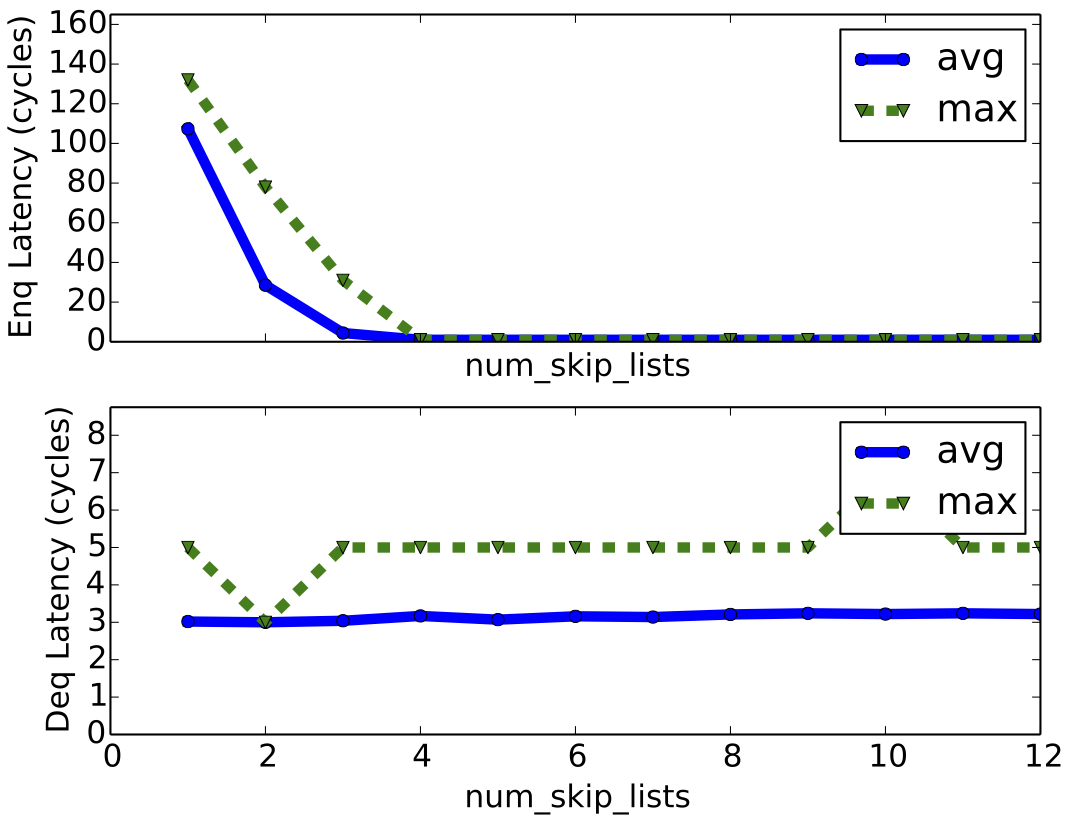
\includegraphics[width=1\linewidth]{figures/eval/enq_deq_v_num_skip_lists}
\caption{Effect of using more parallel skip lists on the enqueue and dequeue latencies.}
\label{fig:num_skip_lists}
\end{figure}


\subsubsection*{Utilization Summary}
We compiled our PIFO onto a Virtex-7 FPGA in order to calculate the resource utilization and verify that the design meets all timing constraints. Table \ref{tab:utilization} provides a summary of the FPGA resource utilization for a single PIFO.

\begin{table}[tbp]
\centering
\caption{Virtex-7 resource utilization for a single PIFO that uses 11 parallel priority queues and has a total capacity of 2K packet descriptors.}
\label{tab:utilization}
\begin{tabular}{|l|l|}
\hline
\multicolumn{1}{|c|}{\textbf{Resource}} & \multicolumn{1}{c|}{\textbf{Utilization}} \\ \hline
LUTs                                    &  51777                                         \\ \hline
FFs                                     &  40586                                         \\ \hline
32Kbit BRAM Tiles                       &  44                                         \\ \hline
\end{tabular}
\end{table}

\subsection{Scheduling algorithm demonstrations}\label{sec:sched-evals}

In this section, we provide the first demonstrations of using a PIFO to implement various common scheduling algorithms. We assume that the rank computation for each scheduling algorithm has already been completed and only concern ourselves with the behavior and evaluation of the scheduling logic. The following evaluations use a single PIFO and packet buffer rather than the full scheduler design in order to minimize the required simulation time. Table \ref{tab:params} shows the design parameters that we used for these evaluations. These demonstrations indicate that our PIFO scheduler is capable of meeting line rate requirements and is flexible enough to be used as a primitive to implement common scheduling algorithms.

\begin{table}[tbp]
\centering
\caption{Parameters used for scheduling algorithm evaluations}
\label{tab:params}
\begin{tabular}{|l|l|}
\hline
\multicolumn{1}{|c|}{\textbf{Parameter}} & \multicolumn{1}{c|}{\textbf{Value}} \\ \hline
PIFO size (pkts)                         & 2048                                \\ \hline
Register Cache Size (pkts)               & 16                                  \\ \hline
Buffer size (64B segments)               & 2048                                \\ \hline
Num Skip Lists                           & 11                                  \\ \hline
\end{tabular}
\end{table}

\subsubsection*{Strict Priorities}

The strict priority scheduling algorithm guarantees that the highest priority queue receives the full egress bandwidth so long as it has any packets in it. This algorithm would be used in scenarios with a limited amount of high priority traffic. In order to implement strict priorities with a PIFO, the rank of each packet is simply equal to its assigned queue ID, where queue 0 is the highest priority queue.

We conducted an experiment where a high-bandwidth low-priority flow is combined with a short flurry of 175 high-priority packets sent at 2 Gb/s. The buffer space is partitioned into two queues and each flow is assigned to a different queue. The aggregate rate of both flows is 10 Gb/s and the PIFO is configured to drain at 4 Gb/s. Figure \ref{fig:strict_queues} shows the size of each queue for the duration of the experiment, and Figure \ref{fig:strict_rates} shows the measured input and output flow rates. We can clearly see that the high priority flow passes through the PIFO scheduler unaffected because its output rate is equal to its input rate, and the high priority queue never contains more than a single packet.

\begin{figure}[!h]
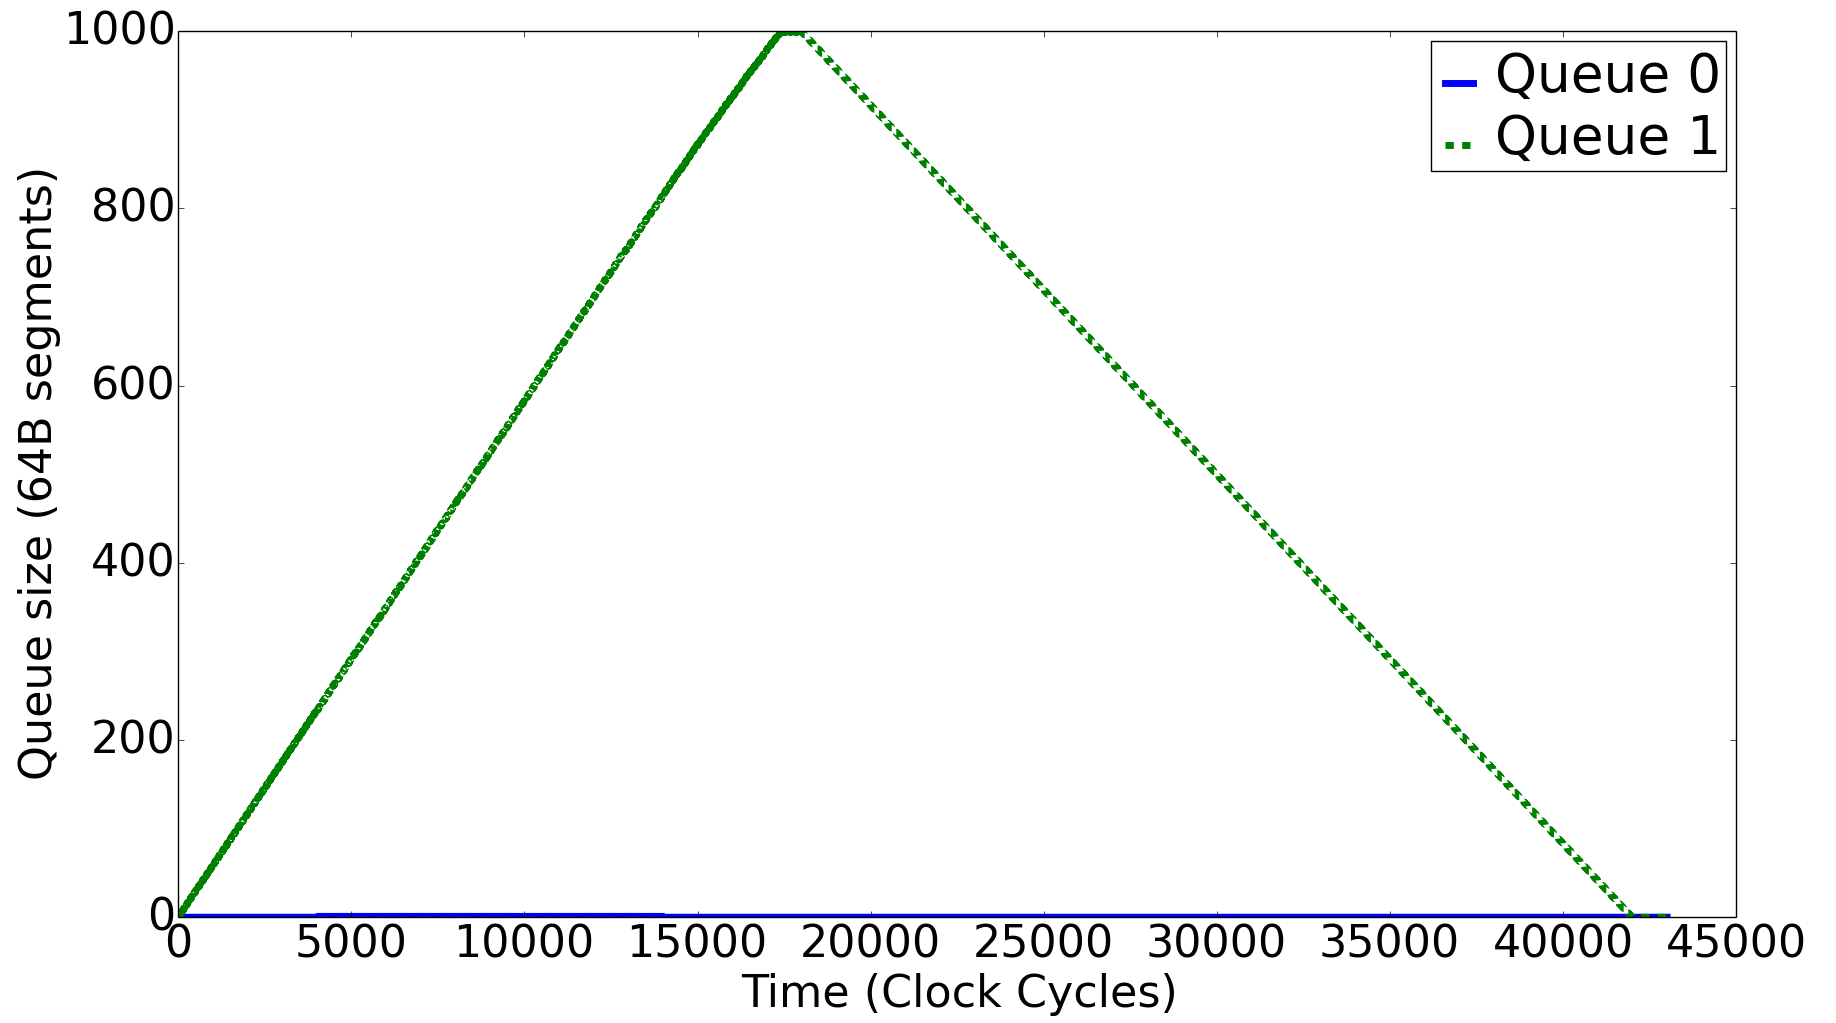
\includegraphics[width=1\linewidth]{figures/eval/strict_queues}
\caption{Queue sizes during strict priority scheduling experiment using our PIFO implementation. Queue 0 is the high priority queue.}
\label{fig:strict_queues}
\end{figure}

\begin{figure}[!h]
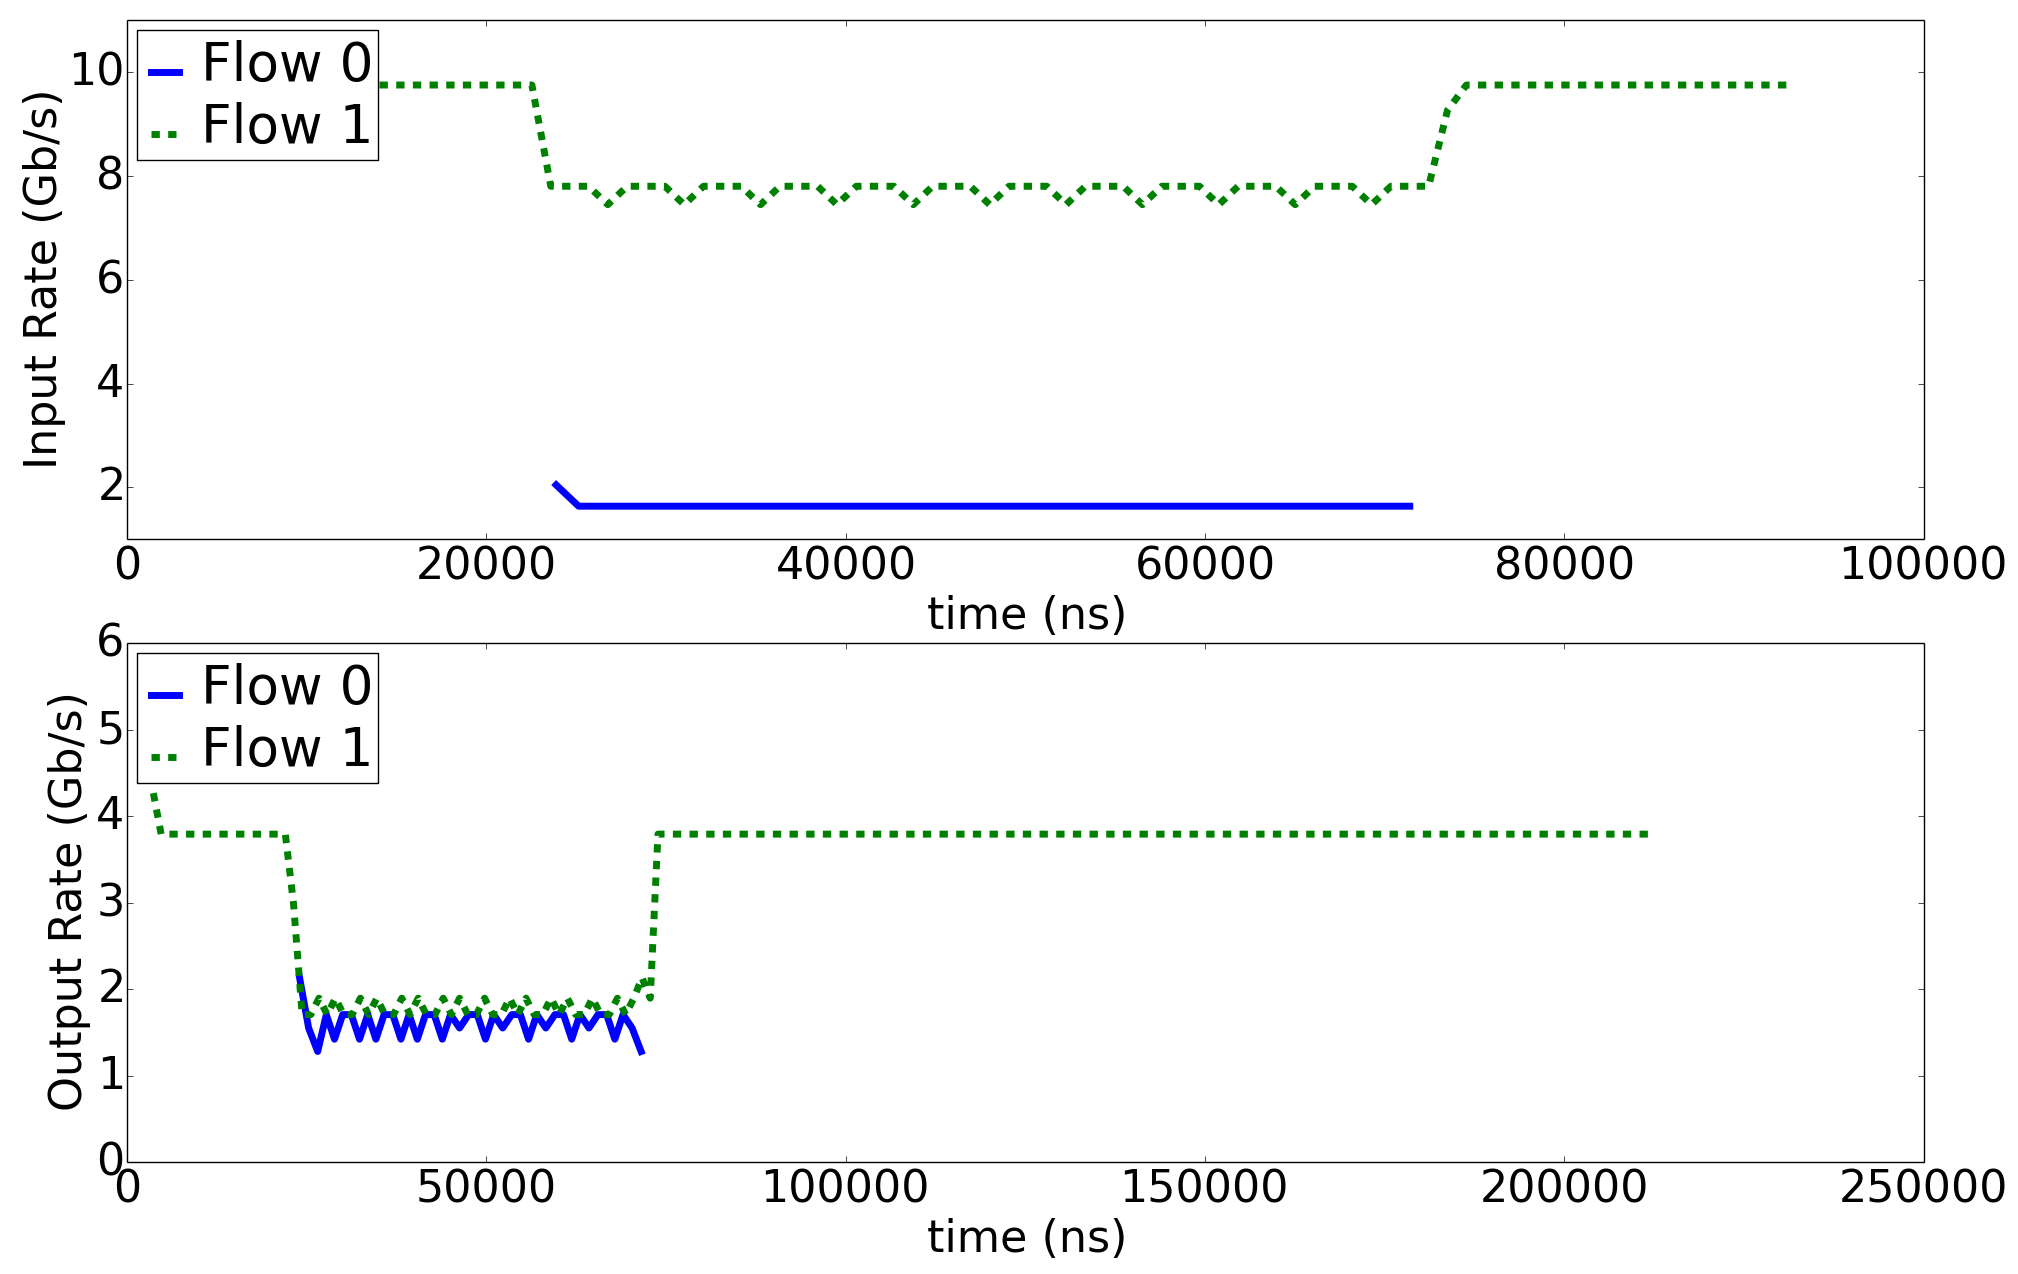
\includegraphics[width=1\linewidth]{figures/eval/strict_rates}
\caption{Strict priority scheduling using our PIFO implementation.}
\label{fig:strict_rates}
\end{figure}

\subsubsection*{Round Robin}\label{sec:round-robin}

Round robin scheduling is the process of serving a single packet from each queue in an alternating fashion. We conducted an experiment using four flows of 64B packets, where each flow has its own queue in the scheduler. The rank of each incoming packet is precomputed to implement round robin scheduling and we measured the input and output rate of each flow. The input rate of each flow is variable, but the total aggregate input rate is 10 Gb/s. The PIFO scheduler is configured to drain at 4 Gb/s. Since all packets are the same size, we would expect round robin scheduling to evenly share the egress bandwidth between all flows. Figure \ref{fig:rr_rates} shows the results of this experiment and indicates that our PIFO scheduler is indeed behaving as expected. Each of the four levels in the output rate plot indicates that the bandwidth is being equally shared between four, three, two, and one flow. The queues do not saturate during this experiment and hence there are no packet drops. This demonstrates that our PIFO scheduler is able to keep up with line rate enqueue operations.

\begin{figure}[!h]
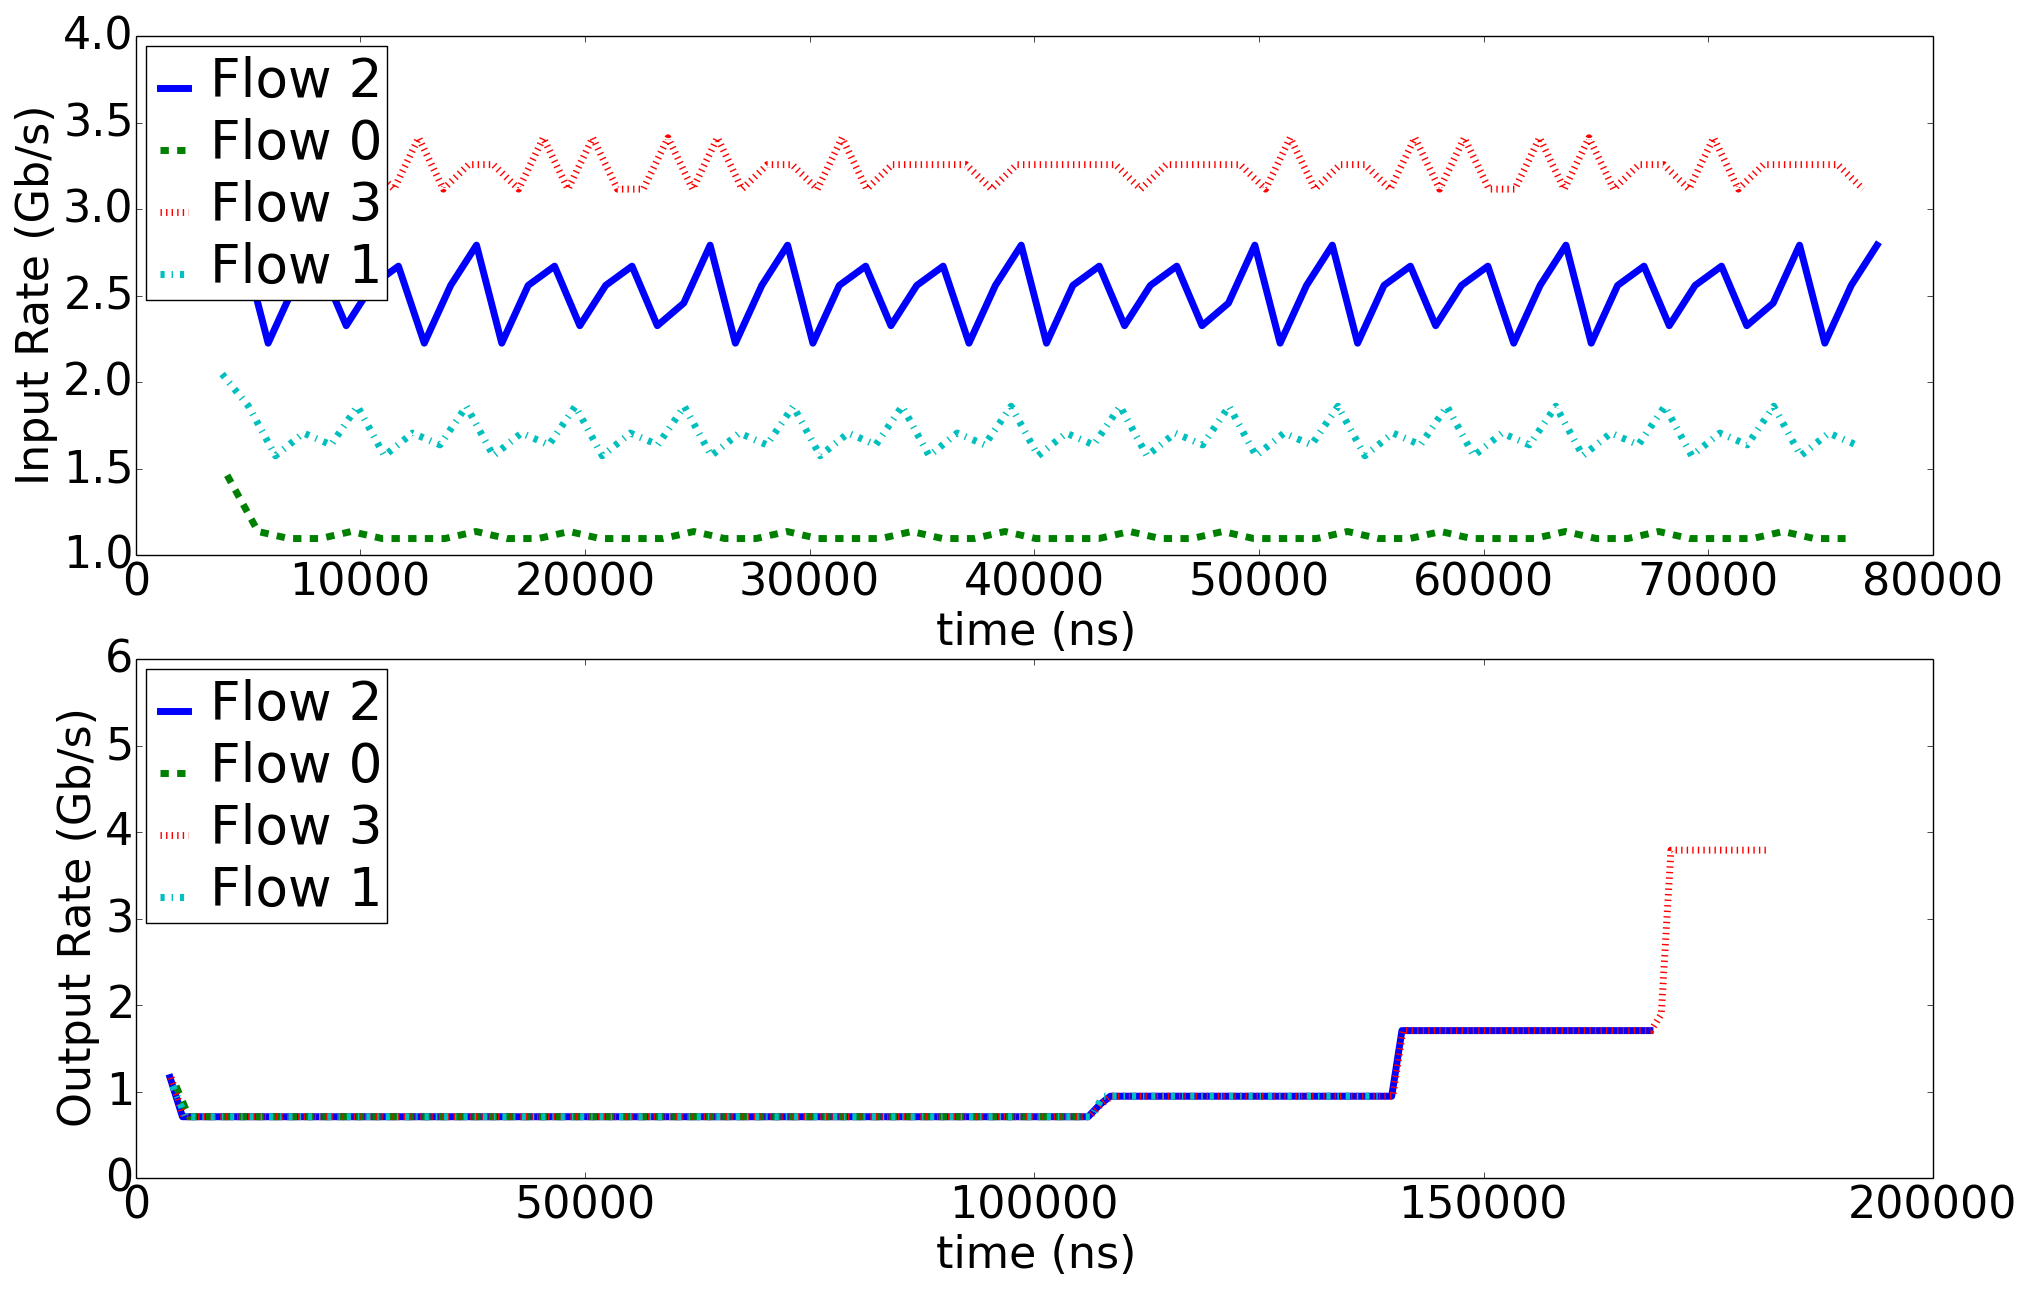
\includegraphics[width=1\linewidth]{figures/eval/rr_rates}
\caption{Round robin scheduling using our PIFO implementation. All flows are sending 64B packets.}
\label{fig:rr_rates}
\end{figure}

\subsubsection*{Weighted Round Robin}

Weighted round robin scheduling is exactly equivalent to round robin if each queue is configured with a weight of one. The queue weights can be configured such that the scheduler dequeues multiple packets from a particular queue according to its weight. We performed the same experiment as the one described in Section \ref{sec:round-robin}, except that the packet ranks are configured to assign to flow 0 a weight that is twice that of the other three flows. Figure \ref{fig:wrr_rates} shows that this weight factor allows flow 0 to pass through the PIFO scheduler completely unaffected by the other three (higher bandwidth) flows.

\begin{figure}[!h]
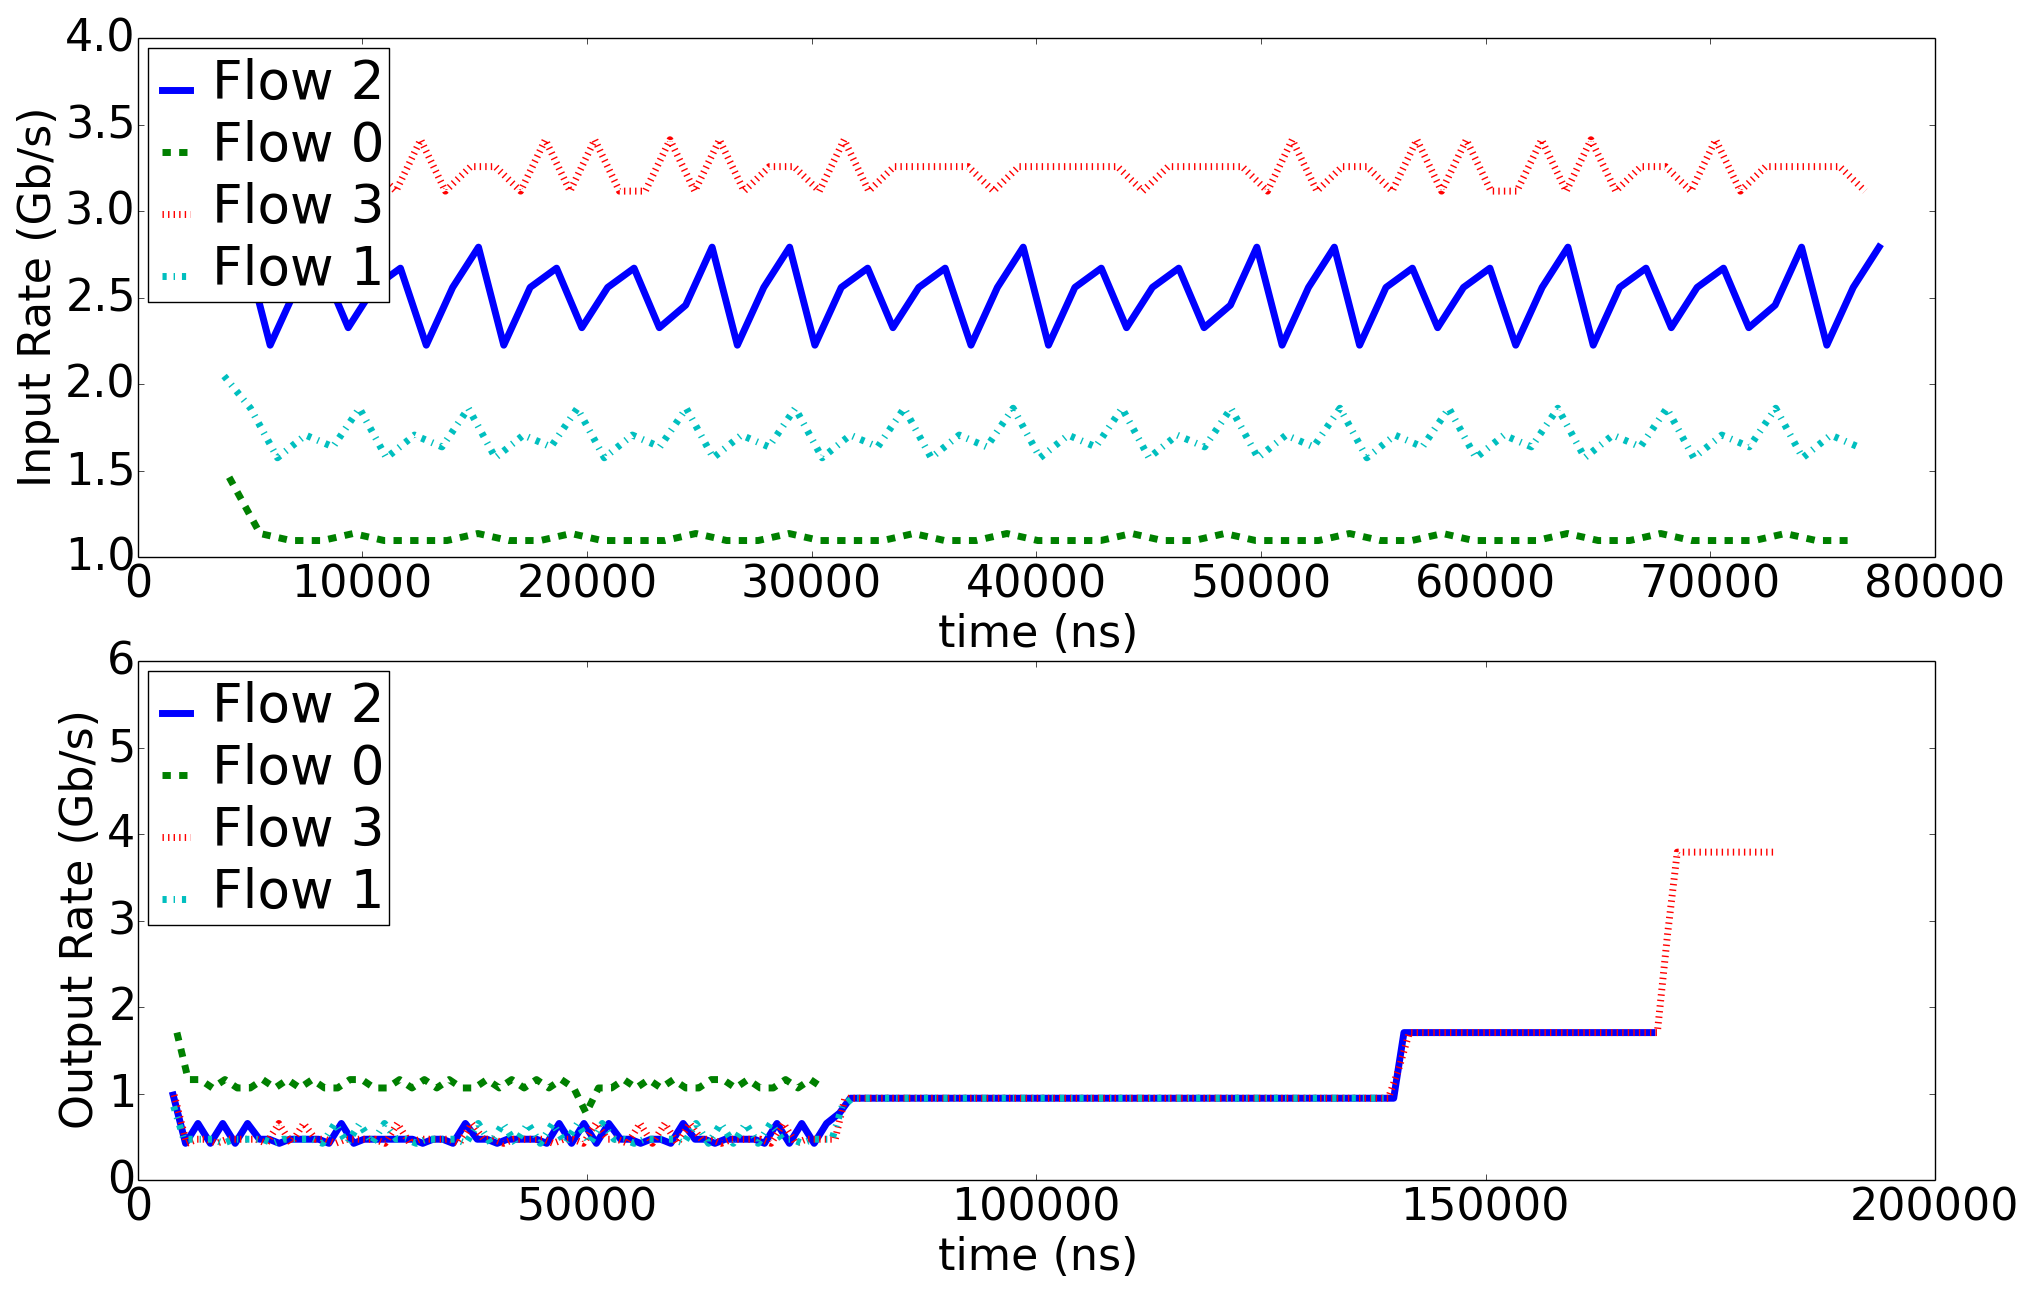
\includegraphics[width=1\linewidth]{figures/eval/wrr_rates}
\caption{Weighted round robin scheduling using our PIFO implementation. All flows are sending 64B packets. Flow 0 is weighted twice as much as the other flows.}
\label{fig:wrr_rates}
\end{figure}

% \subsubsection*{STFQ?}

% \todo[inline]{Needs some debugging}


